\documentclass[xcolor=dvipsnames]{beamer}

\usetheme{Boadilla}

\newcommand{\bi}{\begin{itemize}}
\newcommand{\ei}{\end{itemize}}
\newcommand{\be}{\begin{enumerate}}
\newcommand{\ee}{\end{enumerate}}
\newcommand{\I}{\item}
\newcommand{\f}{\frame}
\newcommand{\ft}{\frametitle}


\begin{document}

\title{GlueX Charged Track Reconstruction Status}
\author[M.\ Ito]{Mark M.\ Ito}
\date{February 27, 2009}

\institute[JLab]{Jefferson Lab}

\f{\titlepage}

\f{
\ft{Detector Diagram}
$$
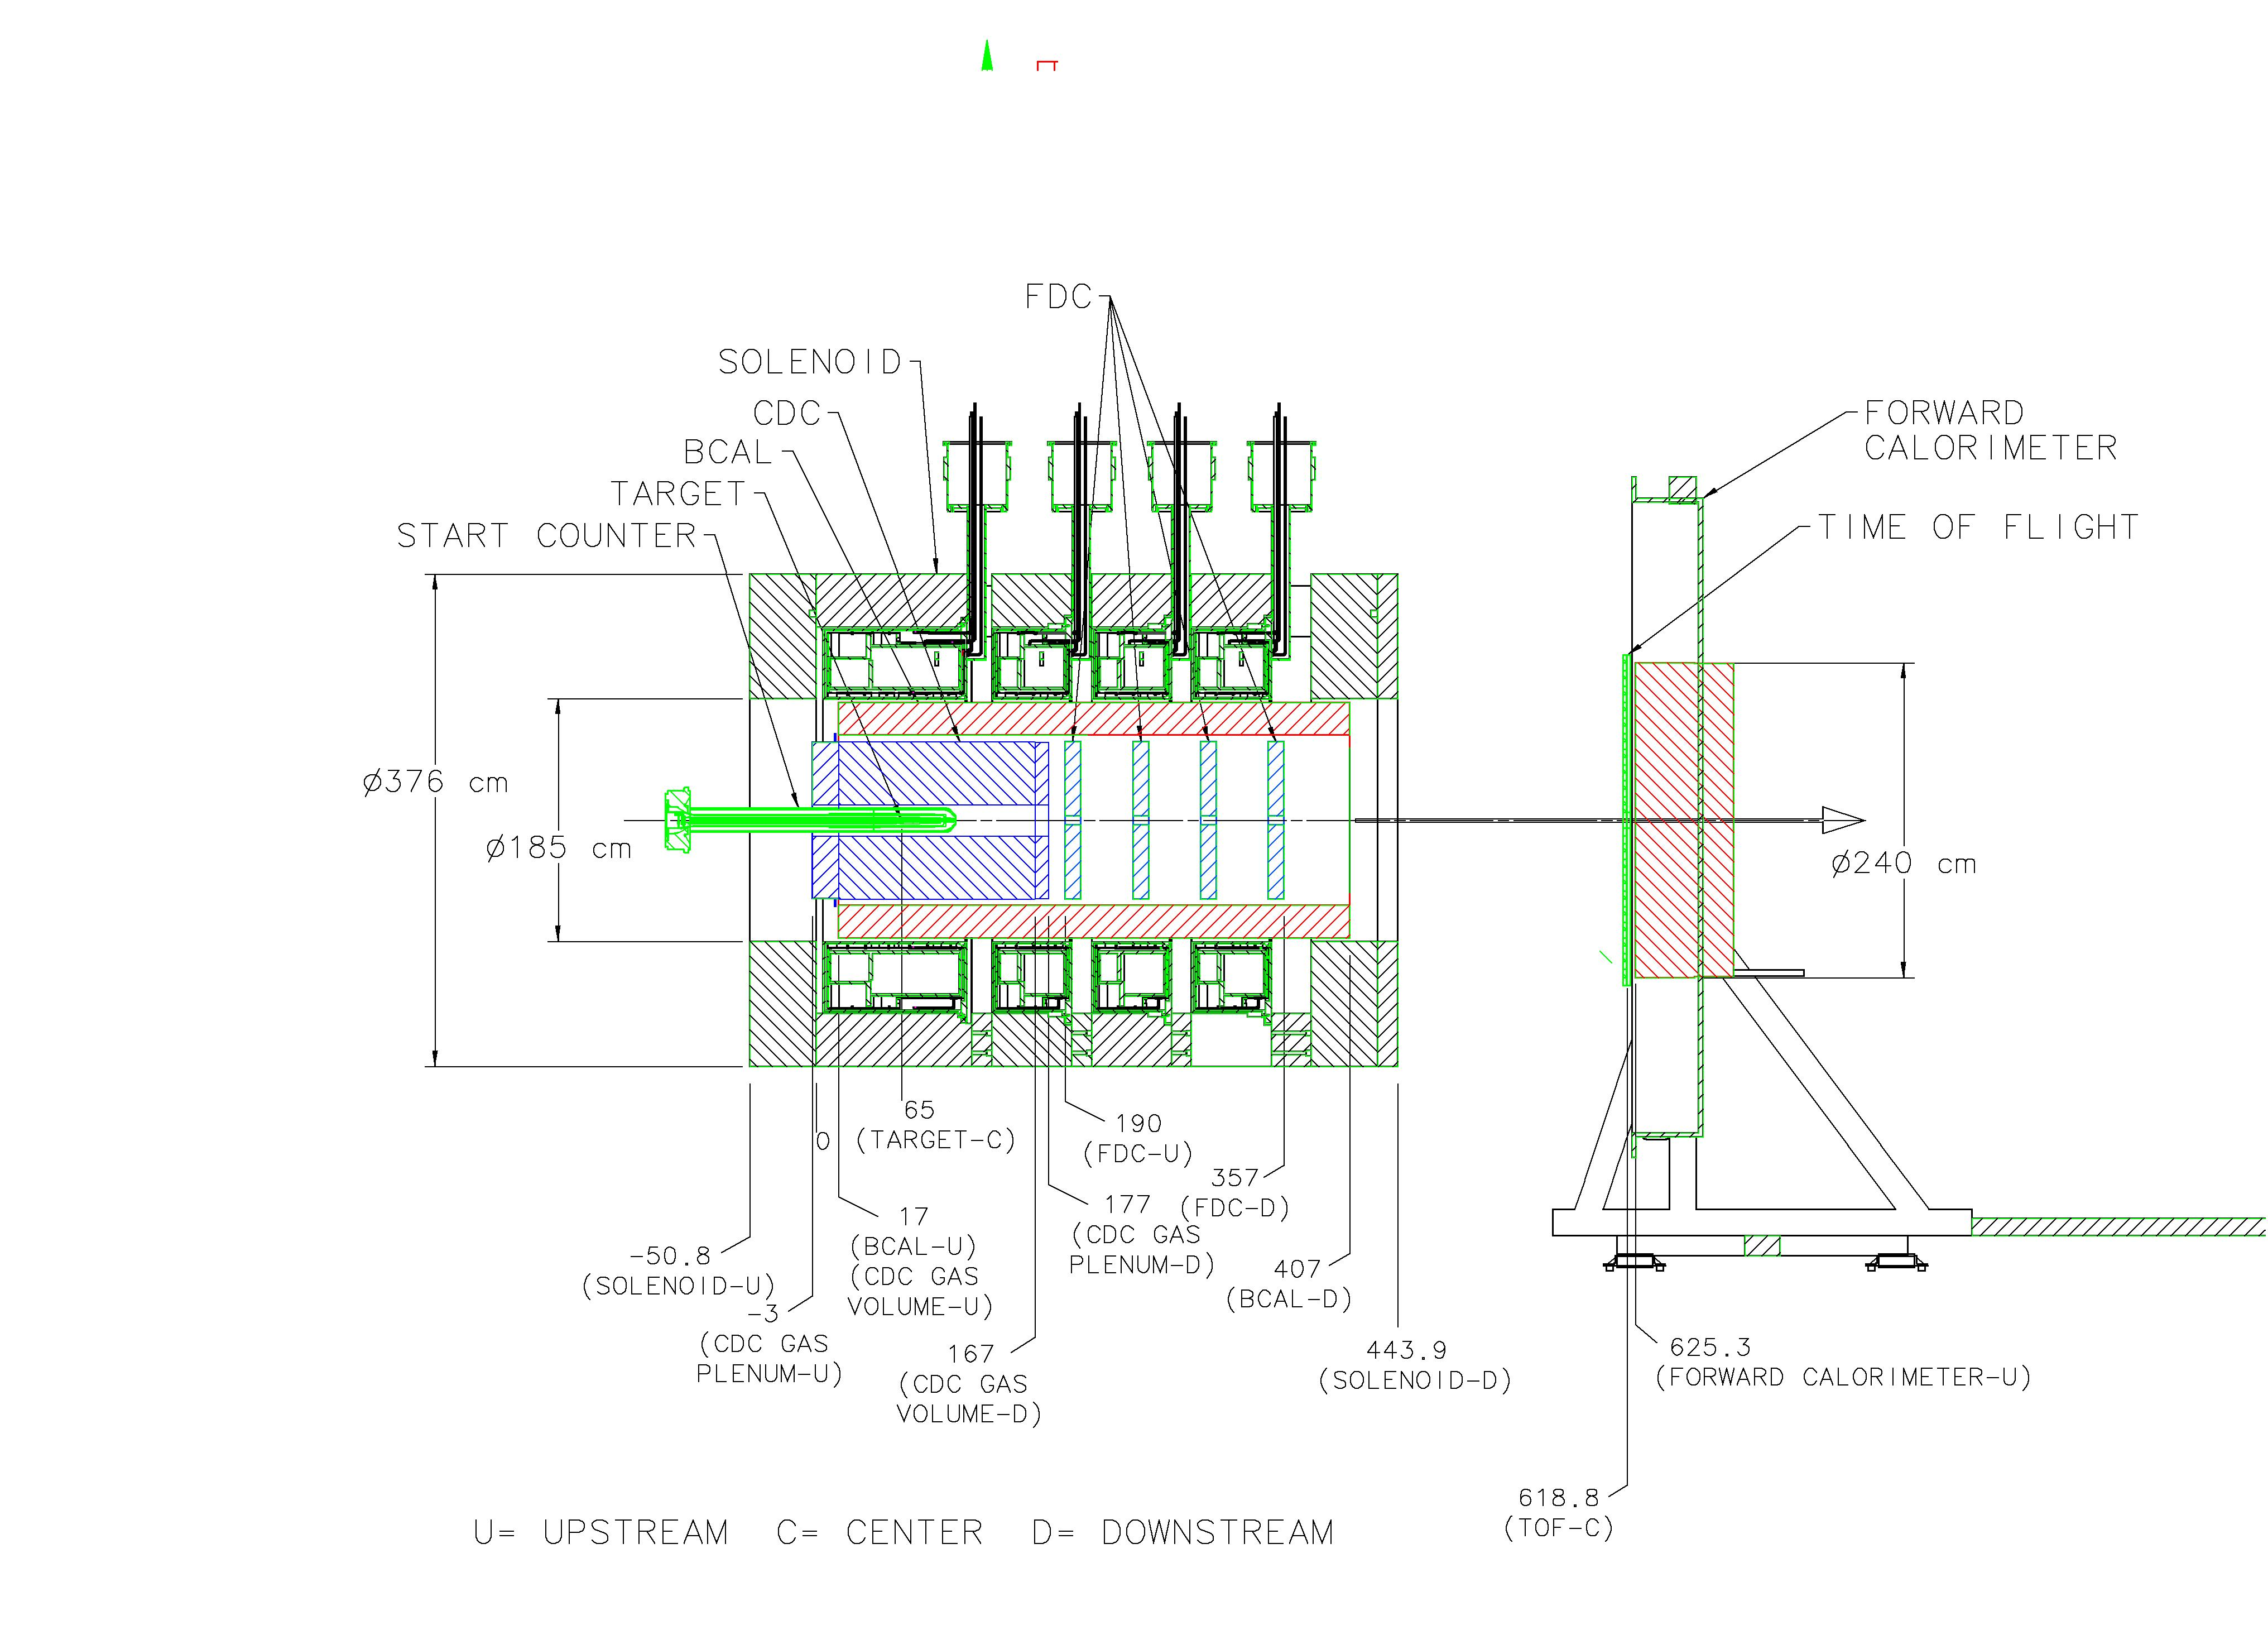
\includegraphics[height=3.0in]{detector.jpg}
$$
}

\begin{frame}[fragile]
\ft{Track Reconstruction}
  \be
  \I Ask for the appropriate vector of objects:
\begin{verbatim}
  vector<const DParticle*>particles;
  eventLoop->Get(particles);
\end{verbatim}
  \I {\tt DParticle} is derived from {\tt DKinematicData}
  \I Both can be found in the {\tt src/libraries/PID} directory
  \I Future work
    \be
    \I multiple track events
    \I improvement in calculation measurement errors
    \ee
  \ee
\end{frame}

\f{
\ft{Track Reconstruction: calling diagram}
$$
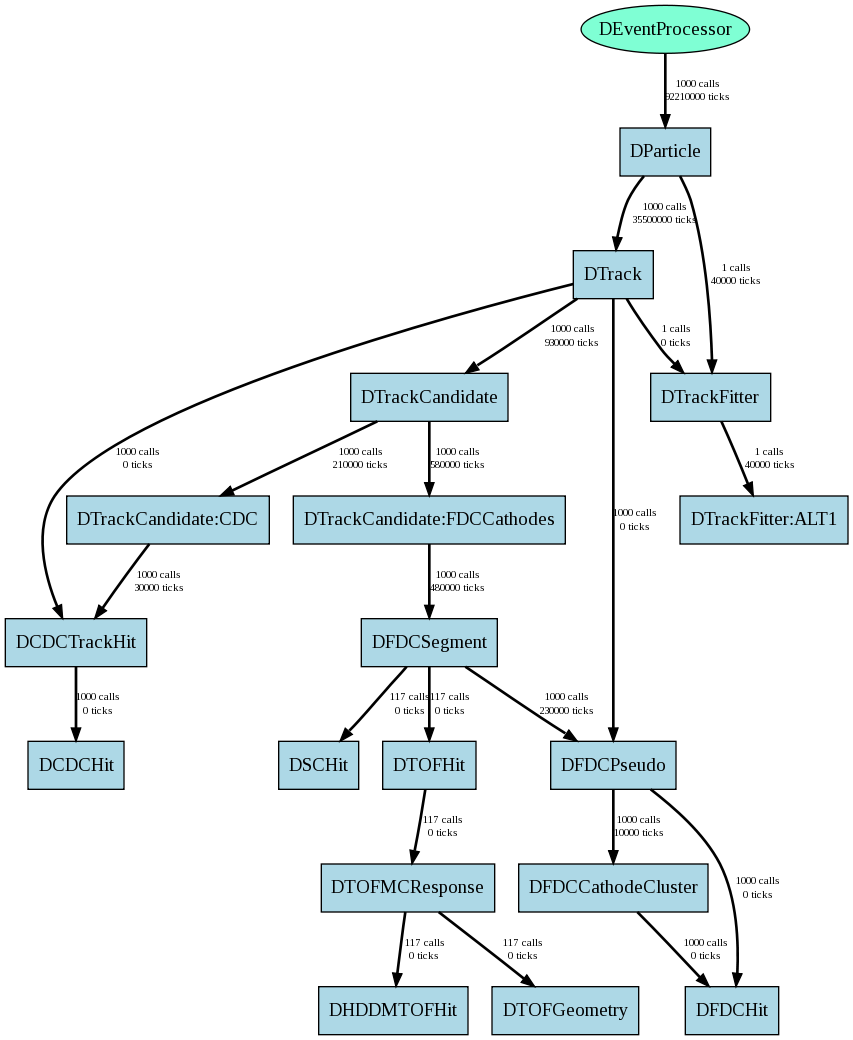
\includegraphics[height=3.0in]{DParticle.png}
$$
}

\f{
\ft{Parametric Monte Carlo}
  \be
  \I Motivation: detector simulation complicated and expensive
  \I Approach
    \be
    \I calculate tables of efficiency and resolution as a function of momentum
    and angles, for charged and neutrals, using full Monte Carlo, in advance
    (experts)
    \I smear ideal 4-vectors by tabulated resolution (user)
    \I fill analyzed vectors with results (user)
    \ee
  \I Main Resource: Wiki page ``HOWTO run the semi-parametric Monte Carlo''
  \ee
}

\f{
\ft{Parametric Monte Carlo: getting started}
  \be
  \I What you need
    \be
    \I Hall D build
    \I checkout and build hdparsim plug-in (see wiki for Subversion repository
    location)
    \I checkout and build any other plug-ins you need (example below)
    \ee
  \I How to run
    \be
    \I generate Monte Carlo events, do not run them through the detector
    simulation ({\tt my\_mc.hddm})
    \I example: {\tt hd\_root --plugin=hdparsim --plugin=invariant\_mass\_hists
      -PDEFTAG:DParticle=HDParSim -PDEFTAG:DPhoton=HDParSim my\_mc.hddm}
    \ee
  \ee
}

\end{document}

%%% end of latex file %%%%
